% !TEX root = Projektspezifikation.tex

\section{Integration}
\subsection{Integrationsprozess}
\subsubsection{Ablauf der Integration}
Die Software wird standardmäßig zwei Quellen integriert haben: die dbSNP und das 1000GenomeProject. Diese werden, über ein Skript gesteuert, heruntergeladen. Wenn dieser Part abgeschlossen ist, wird ein lokaler Parser (später mehr zu den Parsern und ihrer Arbeitsweise) alle relevanten Daten aus den heruntergeladenen Dateien extrahieren und sie in einem, für den globalen Parser akzeptablen Format bereitstellen. Der globale Parser wird diese Dateien dann in Datensätze staffeln und diese dann in das Data Ware House einfügen um sie dann so der Middleware für die Abfragen bereitzustellen.\\
Der lokale Parser wird benötigt, da es kein allgemeingültiges Standardformat gibt, in dem die Dateien abgespeichert werden. Die Formate sind auch keine, von dem DWH anerkannten, Dateiformate, die integriert werden können. Hinzu kommt, dass Sehr viele weitere Daten, die nicht notwendig sind, in den Dateien vorhanden sind und somit nur die benötigten Daten ausgelesen werden müssen.\\
Wenn der User weitere Quellen integrieren möchte, benötigt er zwei Dinge dafür: Ein Downloadskript, welches von der gewünschten Quelle die Dateien herunterlädt, und ein lokaler Parser, der die heruntergeladenen Dateien danach für den globalen Parser bereitstellt.
\subsubsection{Quellenauswahl}
Die Quellen, die von uns integriert sein werden, werden die dbSNP und das 1000GenomeProject sein, da diese alle benötigten Daten frei zugänglich bereitstellen, ohne jegliche Gegenleistung zu verlangen. HGMD hingegen können wir nicht integrieren, da für die Benutzung ihrer Daten eine Lizenz erworben werden muss, die den finanziellen Rahmen des gesamten Projektes sprengt. TCGA konnten wir bei unserer anfänglichen Quellensichtung als "nicht nutzbar" für das Projekt einstufen, da es weder eine Angabe auf ein Referenzgenom gibt, auf das sich die Daten beziehen, noch gibt es Metadaten für die Mutationen. Sollte sich noch eine Möglichkeit ergeben, die Quelle doch integrieren zu können, wird das geschehen, jedoch werden wir uns vorerst auf die frei zugänglichen Quellen konzentrieren, um eine Basis an Daten bereitstellen zu können, weitere Quellen werden im Nachhinein integrierbar sein, weshalb diese Option jederzeit offen steht.
\subsubsection{Attributauswahl und -mapping}
Beide Basis-Datenbanken werden von dem gleichen Anbieter gehostet, was beiden Quellen ein relativ uniformes Format gibt. So stellen beide Quellen die Daten in BAM-Dateien und vcf-Dateien bereit, wobei wir uns auf die vcf-Dateien berufen, da diese die Daten beinhalten, die wichtig sind für die Abfragen, und auch gleichzeitig einfacher zu entschlüsseln sind, als die BAM-Dateien.\\
Wir entschieden uns, dass das Referenzgenom in einer Extradatei abgespeichert wird, um übermäßigen Traffic im DWH zu vermeiden. Des weiteren werden im DWH folgende Daten der Middleware bereitgestellt: Eine einzigartige ID für jeden Eintrag, die Mutationssequenz selber, die Koordinaten, wo im Referenzgenom die Mutation auftritt, der Name der Quelle, um eine schnelle Einordnung nach Quellen zu gewährleisten, der Name des Referenzgenoms, eine Angabe, in welchem Chromosom die Mutation auftritt, und einen Verweis auf den entsprechenden Metadatensatz der Mutation.\\
Der Metadatensatz besteht aus einer eindeutigen ID, der Quelle, woher die Daten stammen, dem Geschlecht des Testsubjekts, dem Herkunftsland und der Downloadzeit. Wir entschieden uns für diese Metadaten, da sie in unseren Standard-Quellen vorhanden sind, und jede nutzbare weitere Quelle auch zumindest diese Daten bereitstellen wird. Die vorhandenen Dateien beherbergen noch eine Fülle weiterer Metadaten, die aber von nur geringer Bedeutung für den eigentlich Zweck unseres Programms sind. 
\subsubsection{Mengengerüst}




%tbd



\subsubsection{Inputfile-Format}
Referenzgenomname:„Name des Referenzgenoms Bsp: GRCh38“\\
Quelle:„hier die Quelle angeben“\\
\$\$\\
SampleID:„hier Samplename“\\
Genkoordinaten:„Angabe der Koordinaten“ \\
Mutationssequenz:„Sequenz“\\
\$\$\\
SampleID:„hier SampleID aus der Datenbank“\\
Gender:„m oder f“\\
Population:„drei Buchstaben bsp: GBR“ \\
EOF\\
\subsubsection{Sequenzdiagramm}
\includepicture[width=\textwidth]{integration/SQDiag.png}{Sequenzdiagramm des Integrationsprozesses\\ Der Ablauf besteht aus zwei Schleifen: Zuerst wird der gesamte Prozess von hinten gestartet, um zu gewährleisten, dass vor Beginn des Integrationsprozesses alle Teilprozesse laufen um Probleme während des Prozesses zu vermeiden. Der globale Parser wird gestartet, startet von sich aus die lokalen Parser, welche dann die Daten ihrer Quelle herunterladen. Nach dem erfolgreichen Herunterladen parsen die lokalen Parser ihre Daten in ein, für den globalen Parser akzeptables Inputfile. Wenn diese Schleife beendet ist, wird der globale Parser alle Inputfiles nehmen und diese dann in das DWH schreiben.}
\subsection{Datenbankentwurf}
\includepicture[width=0.5\textwidth]{integration/DB.png}{Entwurf der Datenbank\\ Die, bereits bei dem Attributmapping genannten, Attribute werden in zwei Tabellen gestaffelt, um eine effizientere und weniger fehleranfällige Struktur zu haben.  Man kann sich möglicherweise sogar Einträge sparen, da es vorkommen kann, dass mehrere Mutationen von der gleichen Person stammen. Außerdem können die Anfragen der Middleware somit auch besser durchgeführt werden.}\\
Erklärungen der Attribute der "Mutation"-Tabelle:\\
\\
\begin{tabular}{|l|c|c|c|c|r|}
Name & Typ & Format & Wertebereich & Beispiel & Notwendigkeit\\
\hline
MutationID & integer & i & 0 - 2.147.483.647 & 1, 2, 3, ...& notwendig\\
\hline
Mutation & text & String & beliebig lang & 'ATTCGATTAGCAGT' & notwendig\\
\hline
Mutationsanfang & bigint & i & 0 - 9.223.372.036.854.775.807 & 60000 & notwendig\\
\hline
Mutationsende & bigint & i & 0 - 9.223.372.036.854.775.807 & 80000 & notwendig\\
\hline
Quelle & text & String & beliebig lang & 'dbSNP' & notwendig\\
\hline
Referenzname & text & String & beliebig lang & 'GRCh38' & notwendig\\
\hline
Chromosom & char(2) & cc & X, Y oder 0 - 99 & 'X', 'Y', '64' & nicht notwendig\\
\hline
MetadatenID & int & i & 0 - 2.147.483.647 & 1, 2, 3, ... & notwendig\\
\end{tabular}\\
\\
Erklärungen der Attribute der "Metadaten"-Tabelle:\\
\begin{tabular}{|l|c|c|c|c|r|}
Name & Typ & Format & Wertebereich & Beispiel & Notwendigkeit\\
\hline
MetadatenID & int & i & 0 - 2.147.483.647 & 1, 2, 3, ... & notwendig\\
\hline
Quelle & text & String & beliebig lang & 'dbSNP', '1000GenomeProject' & notwendig\\
\hline
Geschlecht & char & c & m oder w & 'm', 'w' & nicht notwendig \\
\hline
Herkunft & text & Länderkürzel & Länderkürzel (meist dreistellig) & 'GBR' & nicht notwendig\\
\hline
Downloadzeit & date & dd/mm/yyyy & Bis zum Jahr 5874897 n.Chr. & '24/12/2015' & nicht notwendig, wird aber per Default auf heutigen Tag eingetragen\\
\end{tabular}\\
\\
Wir entschieden uns für diesen Aufbau, da die Abfragen des Users sich in zwei Bereichen unterteilt: Die Mutation selber und die dazugehörigen Metadaten. Eine Separierung dieser beiden Teilgruppen gibt der Middleware mehr Möglichkeiten schneller und effizienter das gewünschte Ergebnis zu finden. Dabei muss aber beachtet werden, dass es noch eine Relation zwischen den beiden Tabellen geben muss, damit jede Mutation genau einen Metadaten-Datensatz zugewiesen bekommt. Dies war der Grund, weshalb wir uns für das relationale Datenbankschema entschieden. Dieses Datenbankschema gibt uns die Möglichkeit, eine Relation zwischen den Mutationen und den Metadaten zu erstellen.\\
Nach dieser Entscheidung benötigten wir ein Datenbankmanagementsystem, was den Ansprüchen des Projektes gerecht werden musste, das heißt, dass es effizient mit großen Datenmengen umgehen können muss. Unsere Entscheidung fiel auf PostgreSQL. Dieses DBMS kann problemlos viele Daten und vor allem große Datensätze speichern und verwalten, was ausschlaggebend für das gesamte Projekt ist.
\subsection{Entwurf des Parsers}
Der lokale Parser wird auf die jeweilige Quelle zugeschnitten sein. Er wird die vorher heruntergeladenen Dateien entpacken, entschlüsseln und danach die relevanten Daten aus den Dateien herauslesen und in einem einheitlichen Format für den globalen Parser abspeichern.\\
Der globale Parser wird die Einheitsdateien der lokalen Parser nehmen, die beinhaltenden Daten in einzelne Datensätze aufteilen und diese dann in der Datenbank abspeichern und sie somit der Middleware bereitstellen.
\subsection{Klassendigramm}
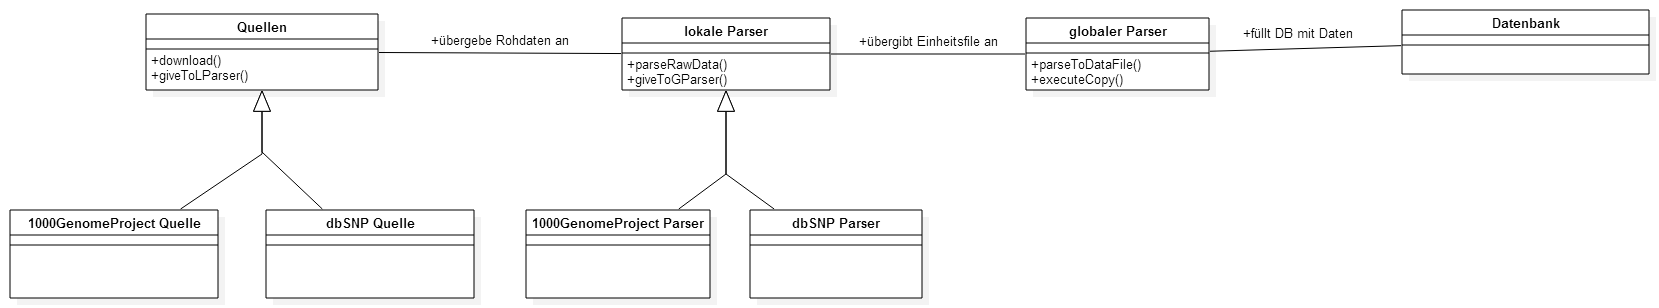
\includegraphics[width=\textwidth]{integration/Klassendiagramm.png}
\subsection{Schnittstellenspezifikation}
\subsubsection{Schnittstelle: Integration - Middleware}
Die Schnittstelle zwischen der Integration und der Middleware ist die, im Modell sichtbare, Datenbank. Sie ist der Ort, an dem die Integration die Daten bereitstellt und von wo die Middleware sich die Daten für die Anfragen abholt.
\subsubsection{Schnittstelle: Integration - Benutzer}
Die Schnittstelle zwischen der Integration und dem Benutzer ist das Hinzufügen neuer Quellen. Der Nutzer wird angehalten sein, zu wissen, wie seine neue Quelle aufgebaut ist, da er selber ein Downloadskript o.ä. dafür schreiben muss, sowie einen lokalen Parser. Diese werden an den entsprechenden Stellen im Programmcode eingefügt. Die lokalen Parser werden durch ein Interface vereinheitlicht.
\subsection{Tests}
\subsubsection{Unit-Tests}
Konkrete Tests konnten wir bisher nicht durchführen, jedoch gibt es einige Dinge zu testen: Es muss getestet werden, ob der lokale Parser arbeitet wie gewünscht, also mindestens 2 Testläufe für ihn: Bei einem, für ihn korrekten Inputfile, muss er ein entsprechend richtiges Outputfile für den globalen Parser erstellen. Sollte er ein Inputfile parsen, was nicht für ihn gedacht ist, soll er das Inputfile verwerfen oder eine Fehlermeldung ausgeben, aber auf alle Fälle das Outputfile nicht mit diesem Input erweitern. Natürlich kann das Inputfile auf verschiedene Weisen korrupt sein, was dort mehrere Testfälle notwendig macht.\\
Der globale Parser muss auf ähnliche Weisen getestet werden, jedoch kann man bei ihm als Voraussetzung annehmen, dass die lokalen Parser korrekt arbeiten und auch ein korrektes Outputfile erstellt haben. Somit müsste nur überprüft werden, dass der globale Parser die Daten korrekt ausliest und korrekt in die Datenbank einfügt.\\
\\
\textbf{Korrektes Inputfile:}\\
\\
Referenzgenomname:GRCh38\\
Quelle:1000Genom\\
\$\$
SampelID:HG0094\\
Genkoordinaten:6:19:19\\
Mutationssequenz: AGTCTAGTA\\
\$\$
SampelID:HG0094\\
Gender:m\\
Population:GRB\\
Download:01:01:2001\\
\\
\textbf{Fehlerhaftes Inputfile}\\
\\
Referenzgenomname:KeinFehlerMöglich\\
Quelle:KeinFehlerMöglich\\
\$\\
SapelID:KeinFehlerMöglich\\
Genkoordinaten:67:21:15\\
Mutationsequenz:ATCERROR\\
\$\$\\
SampelID:KeinFehlerMöglich?\\
Gender:h\\
Population:XXXX\\
Download:64:64:2045\\
